\chapter{Guerra di rete}

«Che schifo Vale! Non mi leccare le orecchie.»

\par\medskip
Laura e Caterina guardano divertite Rocky, che si è già dimenticato di essere stato la causa involontaria delle disavventure delle ultime ore, e saluta Valentina e Alice, sorpreso di trovarle a dormire in soggiorno.

\par\medskip
«Non era mai successo che si allontanasse da solo. Evidentemente deve aver subito il fascino della piccola vagabonda.»

\par\medskip
«Già…»

\par\medskip
Laura guarda l’amica: «Era un sospiro quello?»

\par\medskip
Valentina si stropiccia gli occhi e prova ad abbracciare Rocky, che si sottrae agilmente e si accuccia ai piedi del futon.

\par\medskip
«Rocky! Cos'è successo? State bene?»

\par\medskip
«È una storia lunga, ma dopo ve la raccontiamo.»

\par\medskip
«Sì, ragazze, adesso abbiamo bisogno che ci aiutate. Tra trenta minuti scade la possibilità di salvare il viaggio di Caterina.»

\par\medskip
Alice guarda la sorella.

\par\medskip
«Quindi stai a casa?»

\par\medskip
«No, Ali, aspetta. Forse Laura riesce a sistemare le cose.»

\par\medskip
«Ho bisogno di stare tranquilla qualche minuto per concentrarmi e completare alcune procedure informatiche. Quindi mi raccomando.»

\par\medskip
«Devi hackerare un sito, tatona!»

\par\medskip
«Cosa? Sei anche un'hacker? Ma è fantastico! Sono spariti da più di vent'anni!»

\par\medskip
«Ragazze, è meglio se di queste cose non ne parliamo con nessuno, ok?»

\par\medskip
«Sì, ma niente di speciale, ragazze, vogliamo solo capire perché hanno negato il visto.»

\par\medskip
«Cos’è il rivisto? A proposito, ma ci stiamo dimenticando della...»

\par\medskip
Alice dà un piccolo pizzicotto a Valentina, poi le strizza l’occhio e si avvicina al suo orecchio: «Dai, non dire niente che facciamo una sorpresa alla fine.»

\par\medskip
Valentina ricambia il gesto confidenziale: «Ok» Le conferma e sigilla il patto con un pizzicotto più potente che fa sobbalzare Alice.

\par\medskip
«Ok, va bene. Prepariamo gli strumenti.»

\par\medskip
«Tata ti prego, fai le vocine…»

\par\medskip
«Vale, abbiamo i minuti contati, non ho tempo di giocare...Per questo abbiamo bisogno di:»

\par\medskip
La voce di Laura si fa improvvisamente impostata. Caterina guarda l’amica strizzando leggermente gli occhi e la mette più a fuoco: si chiama sinestesia.

\par\medskip
«…pianificare perfettamente l'operazione. Mappare infrastruttura per identificare i punti deboli e sondare il terreno con una perlustrazione a bassa intensità.»

\par\medskip
Per un attimo, tutto sembra un gioco: i comandi diventano armi, il terminale una mappa, le righe di codice corridoi da attraversare. Ma dietro il tono da soldatesse spaziali, lei sa che la partita è vera: non contro qualcuno, ma contro il tempo.

\par\medskip
«Sì!» Valentina la incita. Alice si avvicina alla sorella e segue la scena con lei.

\par\medskip
Laura esegue una scansione delle porte IP.

\par\medskip
«Bene. Procediamo con un script veloce. Un bel colpo con una \texttt{nmap} nuova di zecca. Carichiamo con un proiettile \texttt{-sS} e puntiamo al 35.228...»

\par\medskip
«Vai Laura!»

\par\medskip
«Fuoco!»

\par\medskip
Laura è decisa e schiaccia il tasto invio con determinazione ma senza forza. La sensibilità è importante. Un comando non deve partire per sbaglio.

\par\medskip
«Bene. Abbiamo colpito. Porte 21 e 80 aperte. Procediamo.»

\par\medskip
Alice sta stringendo la mano a Caterina. Chissà se se ne è accorta o se lo ha fatto automaticamente. Ma intanto che parlo, Laura è già pronta per la sua prossima mossa.

\par\medskip
«Carichiamo \texttt{Hydra} con una lista di stringhe e puntiamo sul bersaglio FTP.»

\par\medskip
«Cosa fai, Tata?»

\par\medskip
«Un attacco di forza bruta, tesoro. Meglio se chiudi gli occhi. Adesso.»

\par\medskip
Attendiamo qualche secondo. Ecco. Ha ottenuto le credenziali.

\par\medskip
«ftpuser/ftppass? Ok. Questo cancella tutti i miei sensi di colpa. La municipale se l’è cercata.»

\par\medskip
Caterina sgrana gli occhi e apre leggermente le labbra. Ma Laura le strizza l’occhio e le sussurra:

\par\medskip
«È un gioco, Cate. Non faremo danni.»

\par\medskip
\begin{center}
  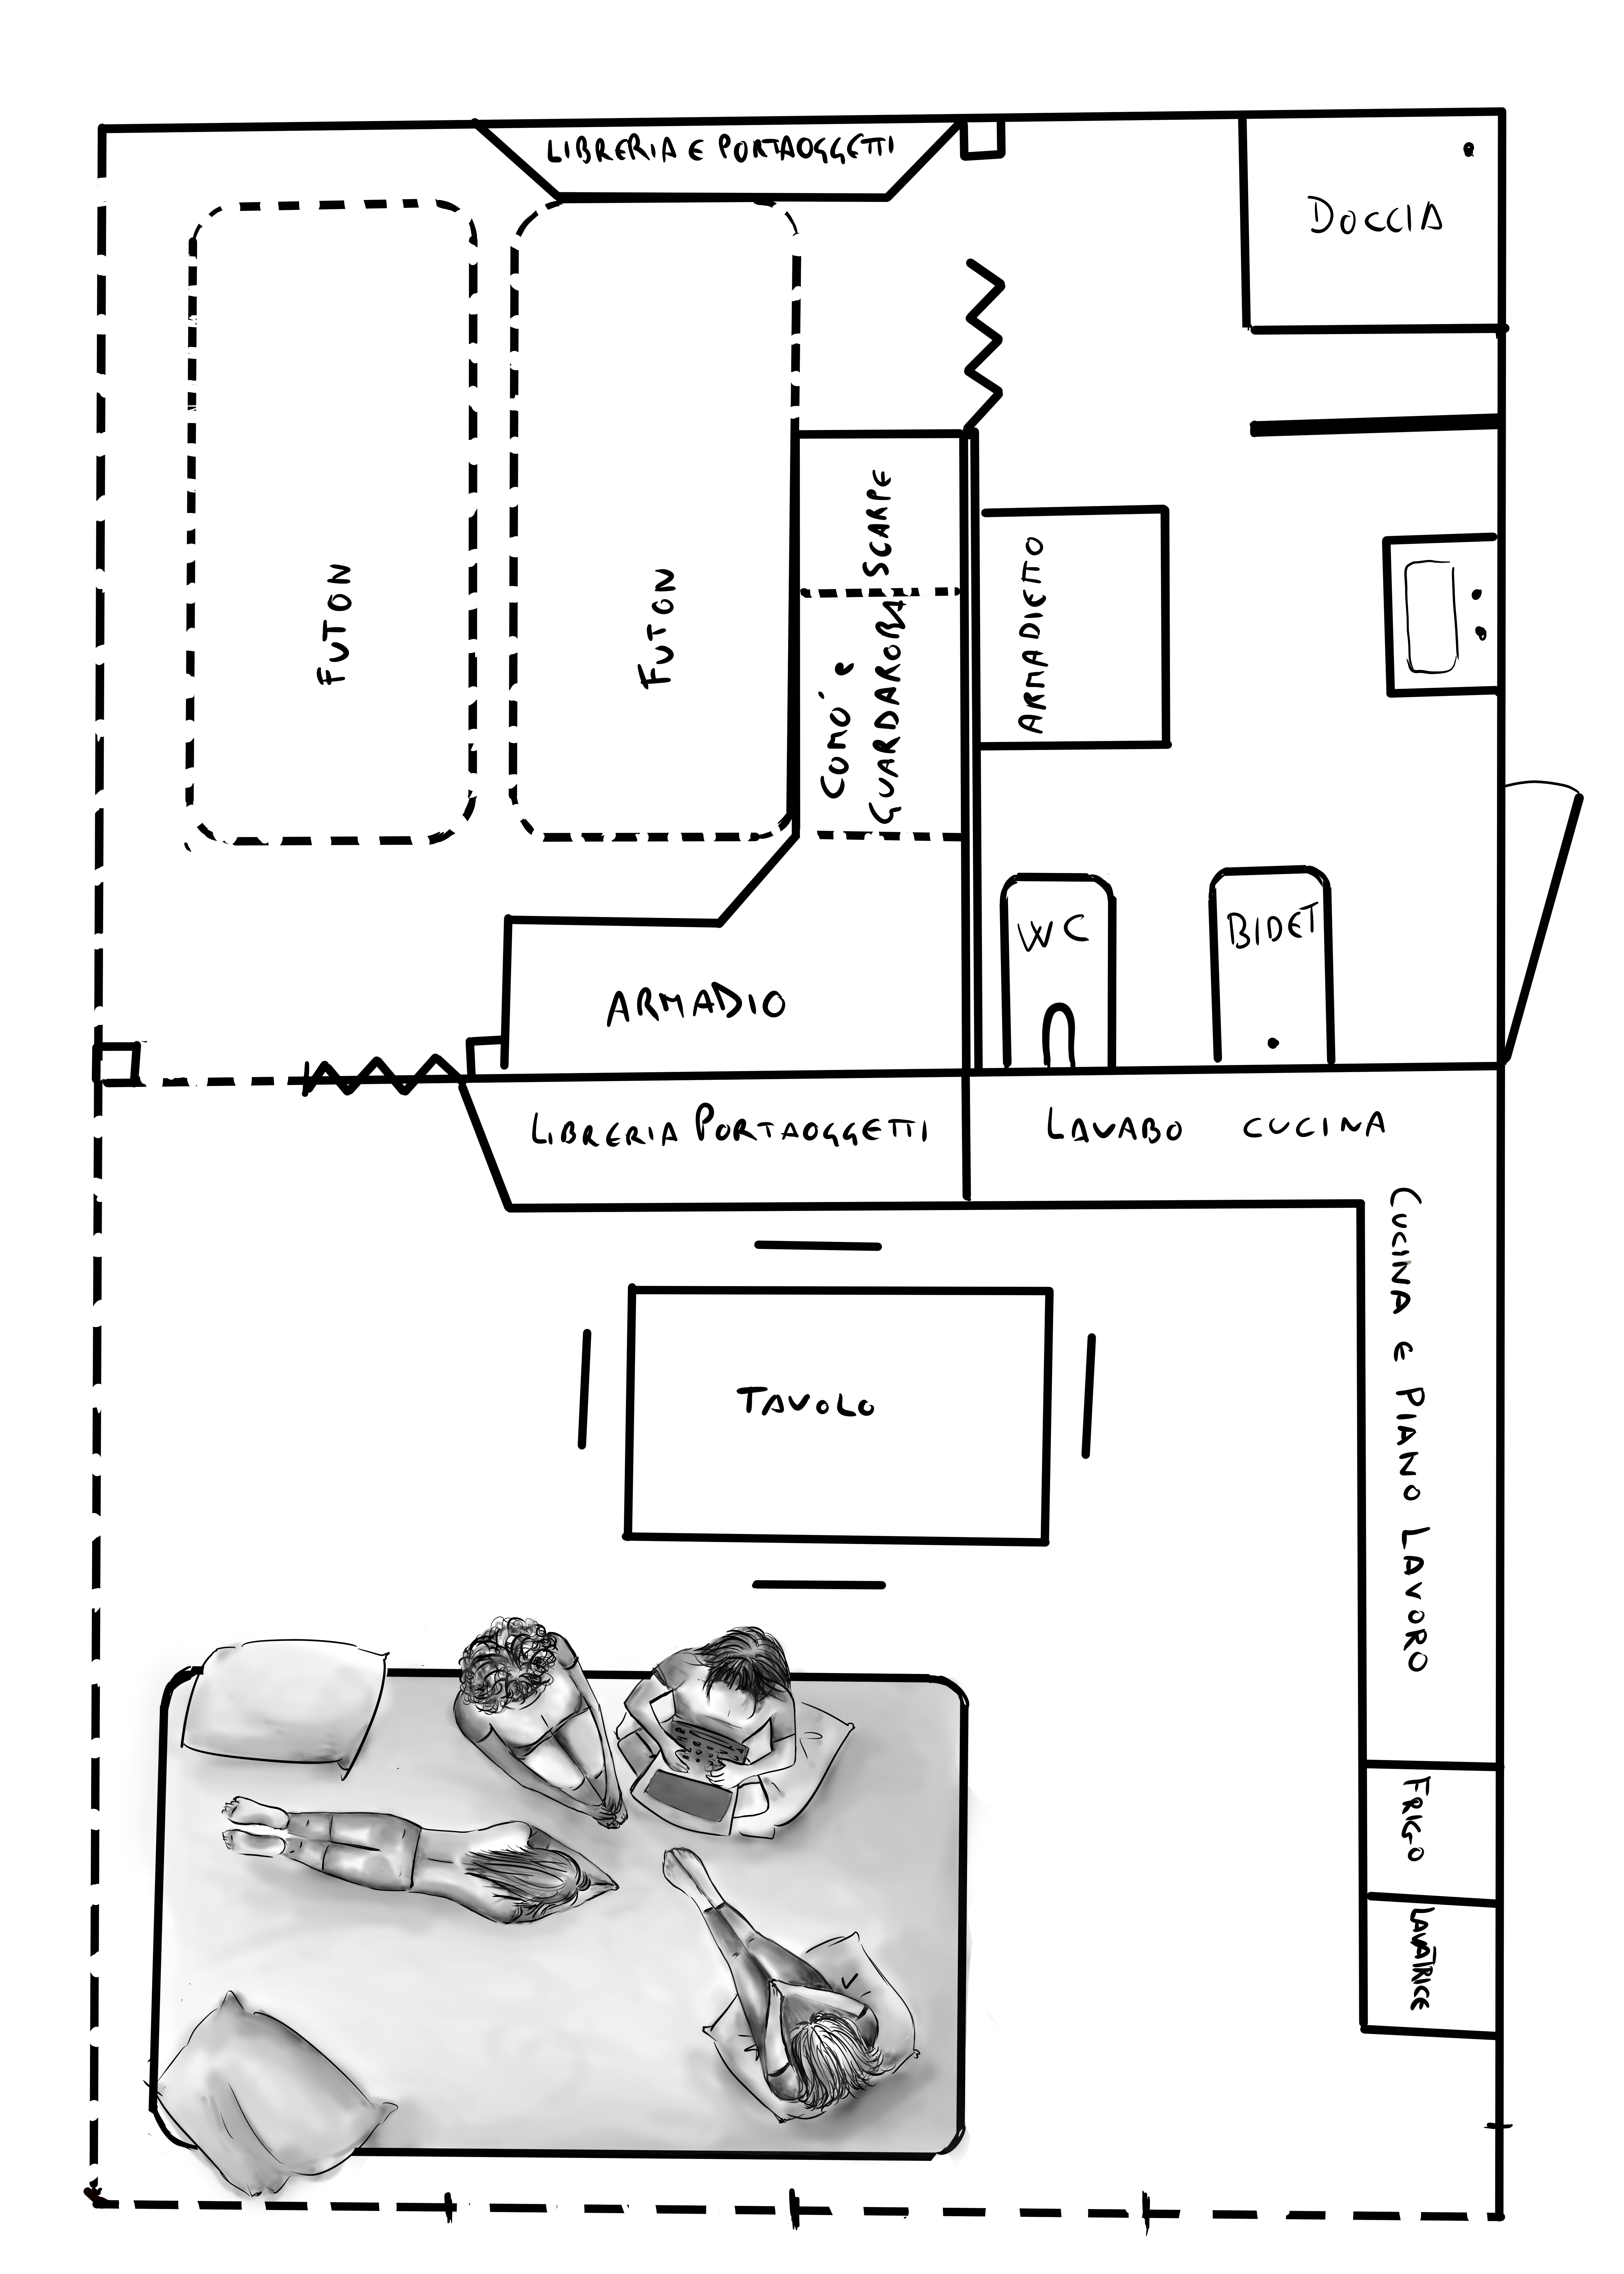
\includegraphics[width=0.7\linewidth]{piantina casa laura senza sfondo.png}
\end{center}

\par\medskip
«Attacco BruteForce sul server 35.228...»

\par\medskip
«Identificate l'IP e geotracciatelo. Vediamo se un pesce cade nella rete.»
